\documentclass{article}
\usepackage[utf8]{inputenc}

% ECS 240 Project Proposal

\usepackage{amsmath}
\usepackage{amssymb}
\usepackage{amsthm}
\usepackage{enumerate}

\usepackage[margin=1.5in]{geometry}

\usepackage{xcolor}
\usepackage{hyperref}
\hypersetup{
    colorlinks,
    linkcolor={red!50!black},
    citecolor={blue!50!black},
    urlcolor={blue!80!black}
}

\usepackage{booktabs,tabularx}
\usepackage{fancyvrb}
\usepackage{tikz}
\usetikzlibrary{arrows.meta,positioning,fit,backgrounds}

% \newcommand{\visiblehref}[2]{\href{#1}{#2}\footnote{\url{#1}}}

\newcommand{\placeholder}[1]{\par\noindent\textit{[TODO: #1]}\par}

\begin{document}

\title{[Project Title]\\\large}
\author{Chang Nguyen \and Nirak Choun \and Nguyen Ho}
\date{}

\maketitle

\section{Introduction and Motivation}

\subsection{Problem Domain and Motivation}

Static program analysis examines program behavior without execution, 
helping detect programming errors such as unreachable code. Cassieri et al. (2022) found 
that developers continued modifying unused or unreachable methods, highlighting the maintenance costs of dead code \cite{paper1}.

However, understanding the causes of programming errors can be challenging. 
Chou et al. (2011) proposed a technique for diagnosing unreachable code in 
hardware verification and suggesting possible fixes \cite{paper2}. Similarly, Feng et 
al. (2026) demonstrated the importance of analyzing execution-path constraints to determine whether vulnerable code is reachable \cite{source3}.

Motivated by these studies, we propose \textbf{PyEye}, an explainable static 
analyzer for a restricted Python-like language. PyEye aims to detect common issues, 
including unused and undefined variables, unused parameters and functions, duplicate declarations, 
and incorrect function argument counts. It will provide clear, human-readable diagnostics explaining 
detected issues and their causes, with unreachable-code detection and more advanced analyses as additional goals.

\subsection{Proposed Language}
\label{sec:proposed-language}
We propose a toy language for writing programs with integer and boolean
expressions, conditional execution, loops, and functions. The language
supports two types: Integers and Booleans.

\subsubsection{Operators}
The language supports the following expression operators:
\begin{itemize}
    \item Arithmetic: \texttt{+}, \texttt{-}, \texttt{*}, and \texttt{/},
    with unary \texttt{-} for negation and parentheses for grouping.
    \item Comparison: \texttt{==}, \texttt{!=}, \texttt{>}, \texttt{>=},
    \texttt{<}, and \texttt{<=}.
    \item Boolean operations: \texttt{!} (negation), \texttt{\&}
    (AND), and \texttt{|} (OR).
\end{itemize}

\subsubsection{Language Constructs}
Programs use \texttt{if}--\texttt{else} for conditional execution and
\texttt{loop} with \texttt{break} for repetition. The language does not
include \texttt{while} or \texttt{for} loops.

The language supports functions, but nested function definitions are not allowed.
Each function has its own scope. Variable lookup first searches the current function's
scope and then the global scope. If a variable is not found in either scope, execution
produces a runtime error.


\subsection{Proposed Tool}

PyEye will be a static analysis tool for our small Python-like
programming language. It will examine source code without executing
it and identify common programming errors. The project will also
include a basic interpreter to execute valid programs.

The static analyzer will support five main features as minimum
requirements:

\begin{itemize}
    \item \textbf{Unused variables:}
    Detect variables that are declared but never read.

    \item \textbf{Duplicate declarations:}
    Detect variables that are declared more than once in the
    same scope.

    \item \textbf{Immutable variable reassignment:}
    Detect attempts to modify variables declared using
    \texttt{let}.

    \item \textbf{Unused functions:}
    Detect functions that are defined but never called,
    excluding the \texttt{main} function.

    \item \textbf{Unreachable code:}
    Detect statements that appear after an unconditional
    \texttt{yeet} statement within the same block.
\end{itemize}

The tool will take PyEye source code as input. It will parse
the code into an Abstract Syntax Tree (AST) and analyze the
program using symbol tables, AST traversal, and basic
control-flow analysis.

For each detected issue, the tool will report its location,
the type of issue, and a short explanation of why it occurs.
Errors will indicate invalid programs, while warnings will
identify potential problems such as unused variables or
functions.

The interpreter will execute PyEye programs according to
the language rules defined in Section~\ref{sec:proposed-language}.


\subsection{Scope and Related Work}
- Muthuraman et al. (2026) reviewed 146 research papers on techniques for optimizing static analysis,
highlighting how existing research focuses on improving execution speed, memory usage, and precision.
While these aspects are important, PyEye takes a different approach by focusing on providing consistent,
understandable diagnostics that explains the issues detected in source code.

- Similarly, Chou et al. (2011) proposed advanced techniques for diagnosing unreachable code in hardware verification.
Their research highlights the importance of identifying and explaining why certain code cannot be executed, rather than
simply detecting it. This motivates PyEye's goal of providing explanations for detected programming issues, including
unreachable statements as a target feature. Unlike their approach, PyEye focuses on simpler static-analysis techniques
for a restricted Python-like language.  

\section{Goals}

\subsection{Minimum Goal}

\begin{itemize}
    \item \textbf{Unused variables:}
    Detect variables that are declared but never read.

    \item \textbf{Undefined variables:}
    Detect variables that are read but never declared.

    \item \textbf{Unused parameters:}
    Detect parameters that are passed in but never read.

    \item \textbf{Duplicate declarations:}
    Detect variables that are declared more than once in the
    same scope.

    \item \textbf{Unused functions:}
    Detect functions that are defined but never called,
    excluding the \texttt{main} function.

    \item \textbf{Wrong argument count:}
    Detect mismatch in argument count when passing arguments into a function.

    
\end{itemize}

\subsection{Target Goal}

No reachable break (IL)

Unreachable statement

\subsection{Reach Goal}

Performance issue detection such as multiple looping

Be able to detect division by 0

\section{Theory Part: Syntax and Semantics}

\subsection{Syntax and Example Programs}

\subsubsection{Syntax}
We used the grammar appendix and the chapter on parsing expressions in
Robert Nystrom's \emph{Crafting Interpreters} as references when drafting
our grammar~\cite{crafting-grammar,crafting-expressions}.

\begin{center}
\begin{BVerbatim}
<prog>           ::= <stmt>*
<stmt>           ::= <block-stmt> | <func-stmt>
<block>          ::= "{" <block-stmt>* "}"
<block-stmt>     ::= <let-stmt>
                   | <assign-stmt>
                   | <if-stmt>
                   | <loop-stmt>
                   | <break-stmt>
                   | <return-stmt>
                   | <expr-stmt>
<let-stmt>       ::= "let" IDENT ("=" <expr>)? ";"
<assign-stmt>    ::= IDENT "=" <expr> ";"
<if-stmt>        ::= "if" "(" <expr> ")" <block> ("else" <block>)?
<loop-stmt>      ::= "loop" <block>
<break-stmt>     ::= "break" ";"
<func-stmt>      ::= "fun" IDENT "(" <param>? ")" <block>
<param>          ::= IDENT ("," IDENT)*
<return-stmt>    ::= "return" <expr>? ";"
<call-expr>      ::= IDENT "(" <args>? ")"
<args>           ::= <expr> ("," <expr>)*
<expr-stmt>      ::= <expr> ";"
<expr>           ::= <or>
<or>             ::= <or> "|" <and> | <and>
<and>            ::= <and> "&" <equality> | <equality>
<equality>       ::= <equality> ("==" | "!=") <comparison> | <comparison>
<comparison>     ::= <comparison> (">" | ">=" | "<" | "<=") <term>
                   | <term>
<term>           ::= <term> ("+" | "-") <factor> | <factor>
<factor>         ::= <factor> ("*" | "/") <unary> | <unary>
<unary>          ::= ("!" | "-") <unary> | <primary>
<primary>        ::= INT | BOOL | IDENT | "(" <expr> ")" | <call-expr>

\end{BVerbatim}
\end{center}

\noindent\textbf{Note:} The grammar allows \texttt{break} outside loops
and \texttt{return} outside functions. These restrictions will need to
be enforced in implementation.

\bigskip

\noindent\textbf{Note:} Whitespace and line comments (starting with
\texttt{//} and continuing to the end of the line) are omitted from
this grammar and skipped during scanning.

\subsubsection{Example Programs}
\paragraph{Expressions and Variables}
\begin{verbatim}
let a = 0;
let b = 1;
let c;
c = a + b;
let ready = (c >= 1) & true | false;
\end{verbatim}

\paragraph{Control Flow}
\begin{verbatim}
fun sum(n) {
  let i = 0;
  loop {
    if (i >= n) {
      break;
    } else {
      i = i + 1;
    }
  }
  return i;
}

let result = sum(3);
\end{verbatim}

\paragraph{Functions and Scope}
\begin{verbatim}
// g is a global variable
let g = 10;

fun foo(a, b) {
  g = a + b;
}

fun main() {
  foo(1, 2);
  // g is now 3
}
\end{verbatim}

\subsection{Semantics Sketch}
\placeholder{In at most one paragraph, sketch the semantics as a set of
(INPUT, prog, OUTPUT) triples. Define the input and output domains and
explain how execution relates them to a valid program. A complete formal
semantics will be required for the final report.}

\section{Implementation Plan}

\subsection{Tool and Language Selection}
The entire pipeline, including the frontend, interpreter, and static analyzer,
will be implemented in Rust.

\subsection{Incorporating Existing Tools}
\placeholder{State which parts will be built from scratch. List any existing
software, libraries, or code bases you will use or interact with, and justify
each dependency.}

\subsection{Architecture of the Code}
The interpreter and static analyzer share a frontend that parses source code
into an abstract syntax tree (AST), as shown below.

\begin{center}
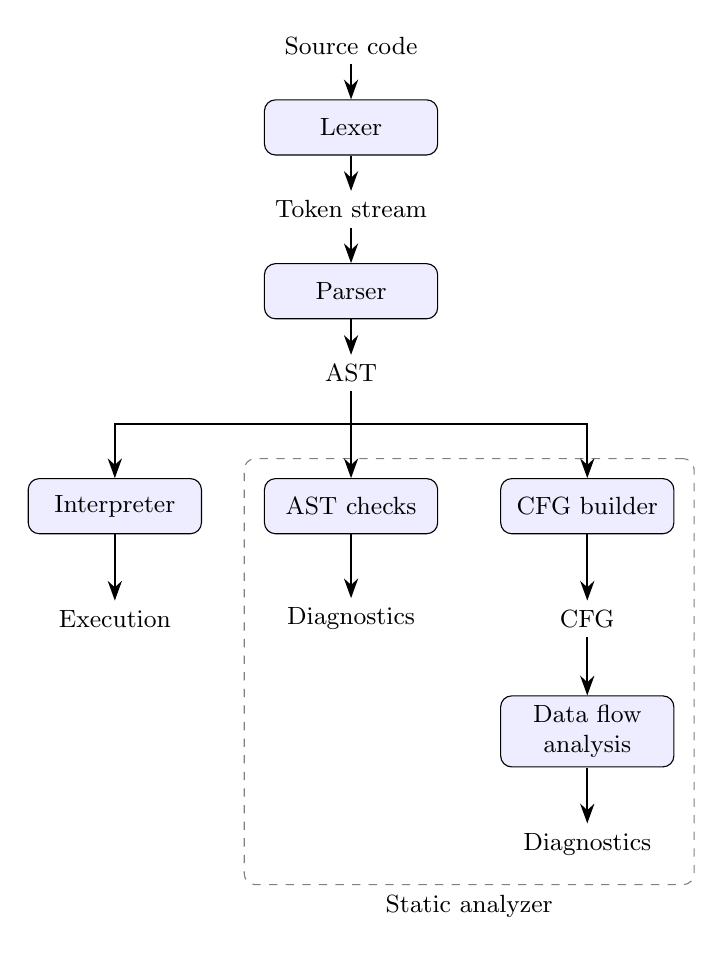
\begin{tikzpicture}[
    font=\small,
    yscale=1.3,
    process/.style={draw, rounded corners, fill=blue!7,
                    minimum width=2.2cm, minimum height=0.7cm, align=center},
    data/.style={align=center},
    flow/.style={-{Stealth[length=2.5mm,width=1.8mm]}, thick}
]
\node[data] (source) at (0,0) {Source code};
\node[process] (lexer) at (0,-0.8) {Lexer};
\node[data] (tokens) at (0,-1.6) {Token stream};
\node[process] (parser) at (0,-2.4) {Parser};
\node[data] (ast) at (0,-3.2) {AST};

\node[process] (interpreter) at (-3,-4.5) {Interpreter};
\node[data] (execution) at (-3,-5.6) {Execution};
\node[process] (checks) at (0,-4.5) {AST checks};
\node[data] (astdiag) at (0,-5.6) {Diagnostics};
\node[process] (builder) at (3,-4.5) {CFG builder};
\node[data] (cfg) at (3,-5.6) {CFG};
\node[process] (dfa) at (3,-6.7) {Data flow\\analysis};
\node[data] (dfadiag) at (3,-7.8) {Diagnostics};

\foreach \from/\to in {source/lexer,lexer/tokens,tokens/parser,parser/ast,
    interpreter/execution,checks/astdiag,builder/cfg,cfg/dfa,dfa/dfadiag}
    \draw[flow] (\from) -- (\to);
\draw[flow] (ast) -- (checks);
\draw[flow] (ast.south) -- (0,-3.7) -| (interpreter.north);
\draw[flow] (ast.south) -- (0,-3.7) -| (builder.north);

\begin{scope}[on background layer]
\node[draw=gray, dashed, rounded corners, inner sep=0.25cm,
      fit=(checks)(astdiag)(builder)(dfa)(dfadiag),
      label={[font=\small]below:Static analyzer}] {};
\end{scope}
\end{tikzpicture}
\end{center}

The code will be organized into one shared library and two binaries.
The frontend will support two error-handling modes: \textbf{error propagation}
and \textbf{error collection}, selected through a Rust feature flag.

In the default mode, \textbf{error propagation}, scanning and parsing errors
propagate through \texttt{Result} return values to the top-level function,
which can either synchronize and continue parsing or return the error to the
caller. The interpreter binary will use this mode.

In \textbf{error collection} mode, diagnostics accumulate in a \texttt{Vec}
during scanning and parsing, with synchronization and continued parsing as
the default behavior. The static analyzer binary will use this mode to report
multiple errors together rather than requiring users to fix them one at a time.

\subsection{Development Effort and Scope}
The planned modules are shown below:
\begin{center}
\begin{BVerbatim}[fontsize=\small]
src/
|-- lib.rs                  # Shared library interface
|-- lexer.rs                # Source code to tokens
|-- parser.rs               # Tokens to AST
|-- ast.rs                  # AST types
|-- errors.rs               # Error reporting and diagnostics
`-- bin/
    |-- interpreter/
    |   |-- main.rs         # REPL and file execution
    |   `-- exec.rs         # AST execution and runtime state
    `-- analyzer/
        |-- main.rs         # Runs checks and reports diagnostics
        |-- cfg.rs          # AST to control flow graph
        `-- dataflow.rs     # Data flow checks over the CFG
\end{BVerbatim}
\end{center}

\placeholder{Map the work to minimum, target, and reach goals, and list
features and components that are out of scope.}

\subsection{Challenges}
Our main challenge is implementing control flow graph (CFG) construction and
data flow analysis (DFA), as we need to fill gaps in our knowledge of these
areas. The initial implementation may have limitations in code quality and
performance, but we will prioritize correctness over optimization.
\bigskip
\placeholder{Expand the challenges and fallback plans after group discussion.}

\section{Collaboration Plan}

\subsection{Division of Work}
\placeholder{Assign components that can be developed separately and explain
how the group will coordinate interfaces, reviews, testing, and integration.}

\begin{center}
\begin{tabularx}{\linewidth}{@{}lX@{}}
\toprule
Group member & Responsibilities \\
\midrule
Chang Nguyen & [TODO: components and responsibilities] \\
Nirak Choun & [TODO: components and responsibilities] \\
Nguyen Ho & [TODO: components and responsibilities] \\
\bottomrule
\end{tabularx}
\end{center}

\subsection{Meetings and Communication}
\placeholder{Specify a meeting schedule (at least twice a week is suggested),
a communication platform, and how you will track tasks and share code.}

\subsection{Weekly Timeline}
\placeholder{Replace the rows below with specific weeks or dates through the
deadline. List deliverables, owners, and dependencies; add rows as needed.}

\begin{center}
\begin{tabularx}{\linewidth}{@{}lXX@{}}
\toprule
Week / dates & Components and deliverables & Owners / dependencies \\
\midrule
{[Week 1]} & [TODO] & [TODO] \\
{[Week 2]} & [TODO] & [TODO] \\
{[Week 3]} & [TODO] & [TODO] \\
{[Week 4]} & [TODO] & [TODO] \\
\bottomrule
\end{tabularx}
\end{center}

\subsection{Commitment Statements}
% Each member should personally sign their statement before submission.
\noindent I commit to work and contribute equally to this project.
\\Name: Chang Nguyen \qquad Signature: \underline{\hspace{1.2in}}

\medskip
\noindent I commit to work and contribute equally to this project.
\\Name: Nirak Choun \qquad Signature: \underline{\hspace{1.2in}}

\medskip
\noindent I commit to work and contribute equally to this project.
\\Name: Nguyen Ho \qquad Signature: \underline{\hspace{1.2in}}

\section{Conclusion and Questions for Feedback}
\placeholder{In one or two paragraphs, describe what success would look like,
what makes the project exciting, and why the application domain matters.
List uncertainties and specific questions for instructor feedback.}

% Mandatory: replace these placeholders with at least three real sources,
% including at least two research papers, and cite them in the text.
\renewcommand{\refname}{References Cited}
\begin{thebibliography}{9}
\raggedright
\bibitem{paper1}
[TODO: Research paper 1 --- authors, title, venue, year, and DOI or URL.]

\bibitem{paper2}
[TODO: Research paper 2 --- authors, title, venue, year, and DOI or URL.]

\bibitem{crafting-grammar}
Robert Nystrom. ``Appendix I: Grammar.'' \emph{Crafting Interpreters}.
\url{https://craftinginterpreters.com/appendix-i.html}.

\bibitem{crafting-expressions}
Robert Nystrom. ``Parsing Expressions.'' \emph{Crafting Interpreters}.
\url{https://craftinginterpreters.com/parsing-expressions.html}.
\end{thebibliography}

\end{document}
